\documentclass{beamer}
% \usepackage{lmodern}
%=====================================================================
% Color definition
\definecolor{jvagreen}{RGB}{0,104,	139}
\definecolor{jvagold}{RGB}{255, 255, 255}
\setbeamercolor{section in head/foot}{fg = jvagold, bg = jvagreen}
\usepackage{graphicx}
\usepackage{mathtools}
\usepackage{picture}
\usepackage{amsmath}
\usepackage{multimedia}
\DeclareMathOperator{\Tr}{Tr}
\graphicspath{{../}}
%\setbeameroption{show notes}
\usepackage{multicol}
\usepackage{caption}
\usepackage{textpos}
\setbeamercovered{dynamic}

\usebackgroundtemplate
{
    
\includegraphics[width=\paperwidth,height=\paperheight]{img/blank.jpg}%
}
\beamertemplatenavigationsymbolsempty

%=====================================================================
% Templates - headline, frametitle

\makeatletter
% Komprimiert die miniframe Kreise auf eine Linie
\beamer@compresstrue
\makeatother

% Definiert die headline
\setbeamertemplate{headline}
{ 
%\includegraphics[width=\paperwidth]{pic} % test logo
\begin{beamercolorbox}[wd=\paperwidth,right]{section in head/foot}
    \rule{\paperwidth}{1pt}
    %Vertikaler Abstand
    \vskip20pt
    %Fügt die Standard-Navi ein (miniframes)
    %\insertnavigation{\paperwidth}
    \vskip8pt
    %\rule{\paperwidth}{0.5pt}
    %\vskip25.5pt % same height of the example provided, but IMHO is too much
    \rule{\paperwidth}{1pt}
\end{beamercolorbox} 
}
\setbeamertemplate{footline}
{ 
%\includegraphics[width=\paperwidth]{pic} % test logo
\begin{beamercolorbox}[wd=\paperwidth,right]{section in head/foot}
    \rule{\paperwidth}{1pt}
    %Vertikaler Abstand
    \vskip10pt
    %Fügt die Standard-Navi ein (miniframes)
    \insertnavigation{\paperwidth}
    \vskip8pt
    \rule{\paperwidth}{0.5pt}
    %\vskip25.5pt % same height of the example provided, but IMHO is too much
    %\rule{\paperwidth}{1pt}
\end{beamercolorbox} 
}

% definition of the frametitle
\setbeamertemplate{frametitle}
{
\vskip-24pt % to shift up the frametitle
\hbox{ 
 \begin{beamercolorbox}[wd=.0675\textwidth]{} % left shift
 \end{beamercolorbox} 
 \begin{beamercolorbox}[sep=4pt]{section in head/foot}
 \insertframetitle
 \end{beamercolorbox} 
 }
}

\mode<presentation>
{
    \setbeamertemplate{itemize item}[circle]
    \setbeamercolor{itemize item}{fg = jvagreen}
    \setbeamertemplate{itemize subitem}[circle]
    \setbeamercolor{itemize subitem}{fg = jvagreen}
}

\renewcommand\footnoterule{}

\AtBeginSection[]
{
  \begin{frame}<beamer>
    \frametitle{Outline}
    \tableofcontents[currentsection]
  \end{frame}
}

%\logo{\includegraphics[height=0.6cm]{img/cde_basic_green}}
%\let\oldequation=\equation
%\let\endoldequation=\endequation
%\renewenvironment{equation}{\vspace{1cm}\begin{oldequation}}{\end{oldequation}\vspace{15mm}}

\begin{document}

\addtobeamertemplate{frametitle}{}{%
\begin{textblock*}{100mm}(-0.9cm,-0.6cm)

\includegraphics[height=0.5cm,width=1.5cm]{img/uob-logo-white-transparent}
\end{textblock*}
\begin{textblock*}{100mm}(0.98\textwidth,-0.6cm)

\includegraphics[height=0.5cm,width=1cm]{img/cde_tag_white}
\end{textblock*}
}

\title[A practical Microcylinder Appearance Model for Cloth Rendering]{
  A practical Microcylinder Appearance Model for Cloth Rendering}

% Optional: a subtitle to be dispalyed on the title slide
% \subtitle{Show where you're from}
% \subtitle{Presented by: Ieva Kazlauskaite}
% The author(s) of the presentation:
%  - again first a short version to be displayed at the bottom;
%  - next the full list of authors, which may include contact information;
\author[Garoe Dorta Perez]{
   Presented by Garoe Dorta Perez } 


% The institute:
%  - to start the name of the university as displayed on the top of each slide
%    this can be adjusted such that you can also create a Dutch version
%  - next the institute information as displayed on the title slide
\institute[University of Bath]{
University of Bath \\
Centre For Digital Entertainment
}

% Add a date and possibly the name of the event to the slides
%  - again first a short version to be shown at the bottom of each slide
%  - second the full date and event name for the title slide

%\date{Presented by Ieva Kazlauskaite, 30 April 2015}

% TITLE PAGE
\begin{frame}[plain]
  \titlepage
\end{frame}

%\section{Overview}
% CONTENT PAGE
\begin{frame}
  \frametitle{Overview}
  \tableofcontents
\end{frame}

%----------------------------------------------------------------------
\section{Introduction}
\subsection{ }
%\begin{frame}{Introduction}
%\begin{itemize}
%\setlength\itemsep{0.5em}
%\item Rendering images realistically
%	\begin{itemize}
%	\setlength\itemsep{0.5em}
%	\item Computationally expensive for large or complex scenes
%	\item Tradeoff between speed and quality
%	\end{itemize}
%\end{itemize}
%\end{frame}

\begin{frame}{Introduction}
\begin{equation*}  
L_o (\mathbf{p}, \boldsymbol{\omega_o}) = L_e(\mathbf{p}, \boldsymbol{\omega_o}) + \int_\Omega f(\mathbf{p}, \boldsymbol{\omega_o}, \boldsymbol{\omega_i}) L_i(\mathbf{p}, \boldsymbol{\omega_i}) | \cos \theta_i | d \boldsymbol{\omega_i}
\end{equation*}

\begin{multicols}{2}
\begin{figure}[b!]
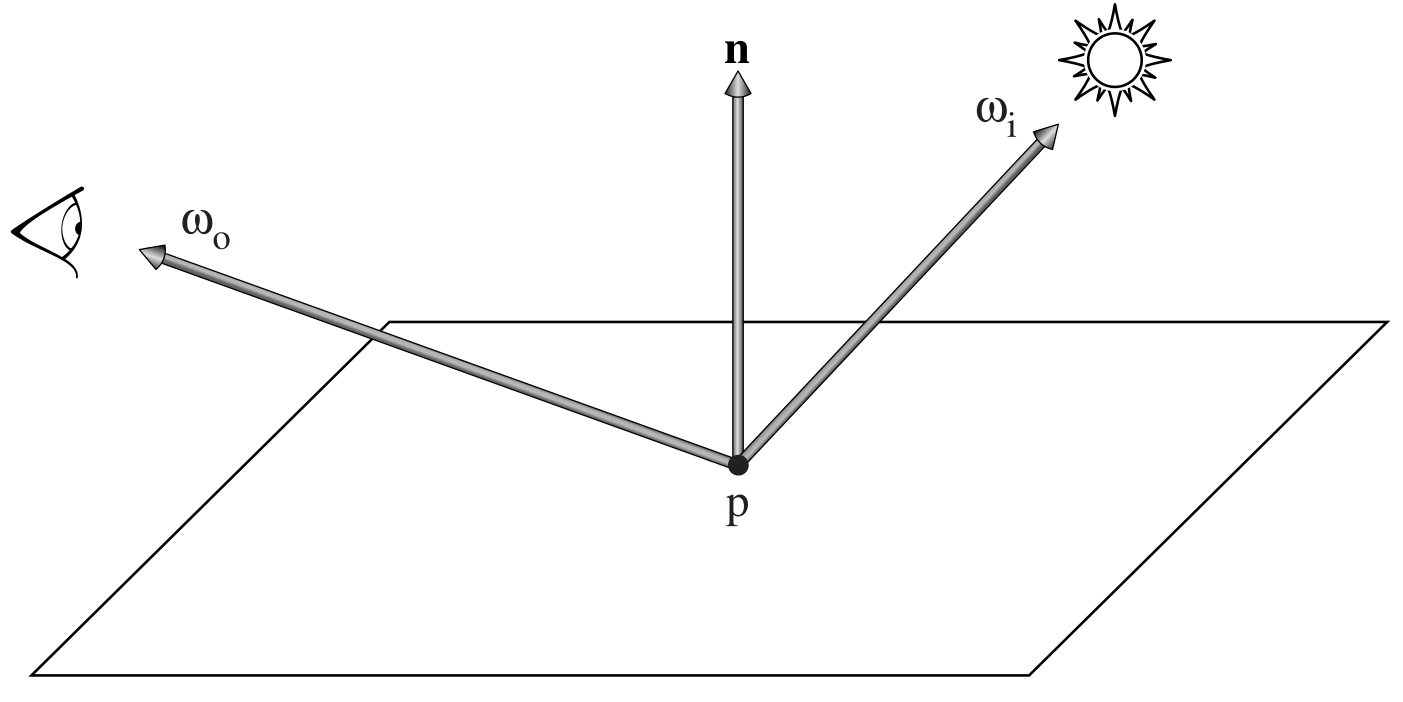
\includegraphics[width=0.5\textwidth]{img/render_definition}
\caption*{\tiny{Diagram of light emitted from $\mathbf{p}$, image taken from [PH10].}}
\end{figure}

\vfill
\columnbreak
\vspace*{\fill}
\small{where $L_o$ is the outgoing radiance, $L_i$ incoming radiance, $L_e$ emitted radiance, $f$ BRDF function, $\mathbf{p}$ surface point, $\boldsymbol{\omega_i}$ incident light, $\boldsymbol{\omega_o}$ outgoing light, $\Omega$ hemisphere above $\mathbf{p}$, $\theta_i$ angle of incidence. }
\end{multicols}
\end{frame}

%\begin{frame}{Main theme: Path tracing approach 1}
%\note{As you know, path tracing bla bla}
%\begin{itemize}
%\setlength\itemsep{0.5em}
%\item Monte Carlo path tracing
%\end{itemize}
%\begin{center}
%\begin{figure}
%\includegraphics[width=0.7\textwidth]{img/path_tracing}
%\caption*{\tiny{Diagram of simple path tracing from eye to light source, image taken from [PH10].}}
%\end{figure}
%\end{center}
%\end{frame}

%\subsection{Cloth rendering}
%\subsection{Appearance models}
\begin{frame}{The problem}
\begin{itemize}
\setlength\itemsep{0.5em}
\item Render cloth fast and realistically 
		\begin{itemize}
		\setlength\itemsep{0.5em}
		\item Small threads
		\item Weaving patterns
		\end{itemize}
\end{itemize}
\begin{figure}[t!]
\begin{center}
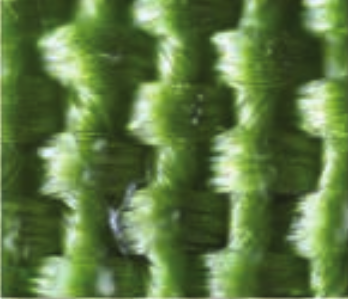
\includegraphics[width=0.4\textwidth]{img/cloth_real} 
~
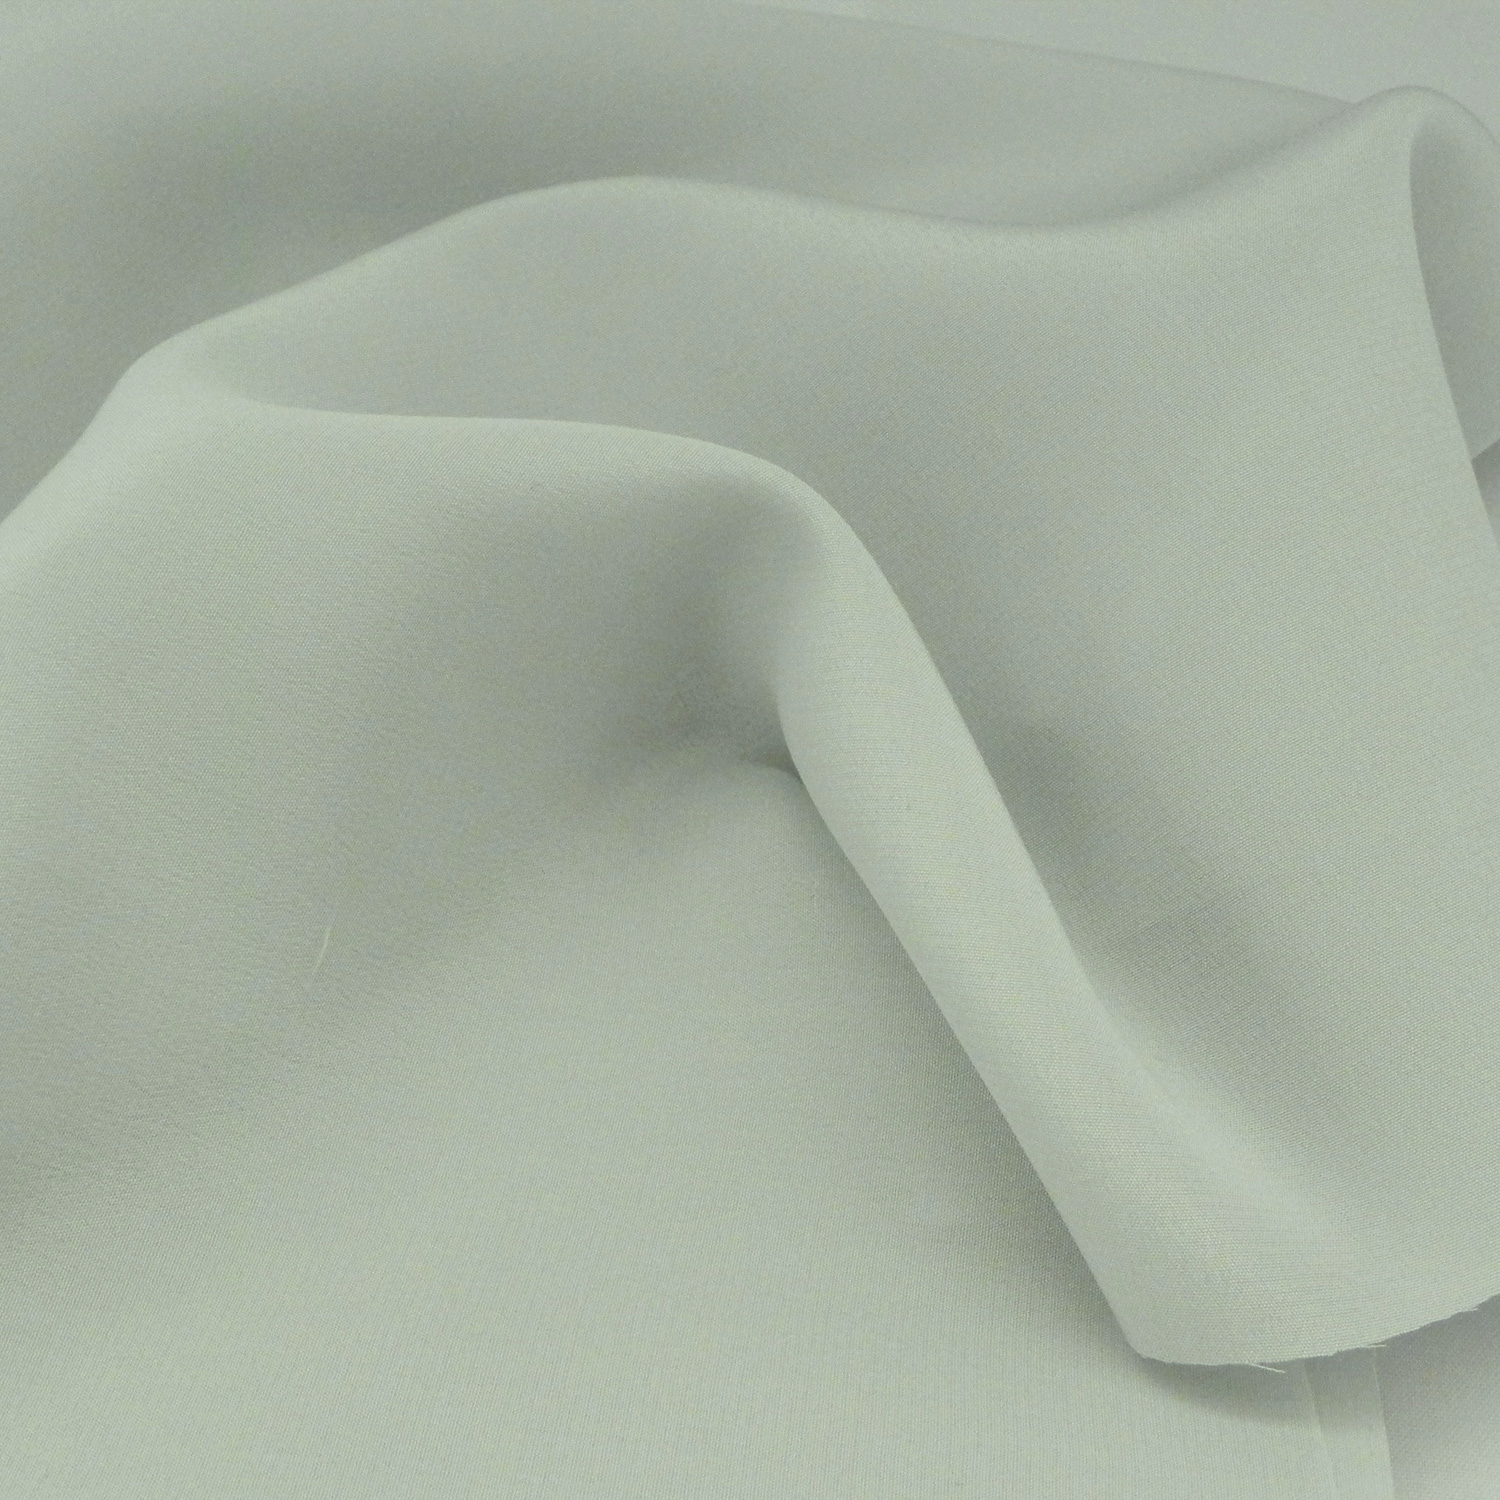
\includegraphics[width=0.4\textwidth]{img/cloth_reference}
\caption*{\tiny{Left shows a close up view of fabric, right shows a picture of cloth, images taken from [SBD*13].}}
\end{center}
\end{figure}
\end{frame}

\begin{frame}{Appearance model}
\begin{itemize}
\setlength\itemsep{0.5em}
\item Two microcylinders [SBD*13]
\end{itemize}
\begin{center}
\begin{figure}
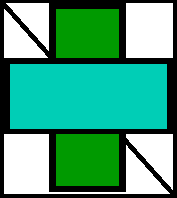
\includegraphics[width=0.4\textwidth]{img/cloth_model}
~
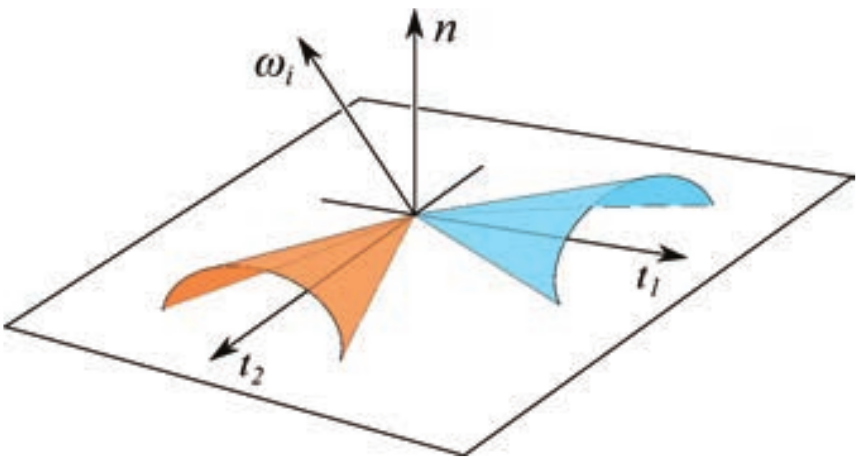
\includegraphics[width=0.5\textwidth]{img/microcylinders}
\caption*{\tiny{Left shows model in a triangle mesh, right shows scattering cones in a patch, images taken from [SBD*13].}}
\end{figure}
\end{center}
\end{frame}

\begin{frame}{Appearance model}
%L_r = L_e + \int_{\Omega} f(t, \omega_i, \omega_r) L_i cos(\theta) \delta \omega_i, \\
\begin{equation*} 
\mbox{BRDF: } f(t, \omega_i, \omega_r) =  \frac{\mbox{Reflection term} + \mbox{Volume scattering term}}{\mbox{Normalization factor}},
\end{equation*}

\begin{multicols}{2}

\begin{figure}[!htb]
    \centering
    \begin{minipage}{.5\textwidth}
        \centering
        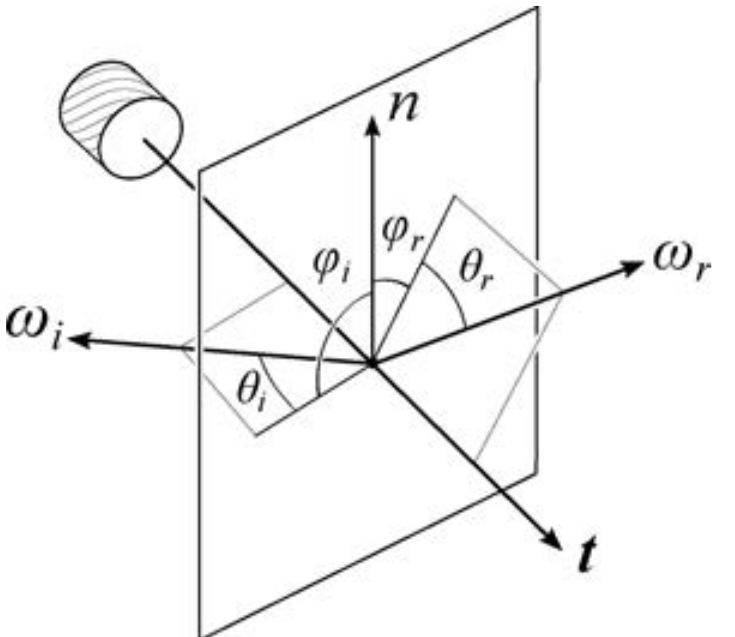
\includegraphics[width=0.8\textwidth]{img/cloth_directions}
        \caption*{\tiny{Angle definitions for a single thread, image taken from [SBD*13].}}
    \end{minipage}%
\end{figure}

\vfill
\columnbreak
\vspace*{0.2cm}
\footnotesize{ where $f$ is the BRDF function, $t$ is the thread direction, $\omega_i$ is the ray incoming direction, $\omega_r$ is the ray outgoing direction. }
\end{multicols}

\end{frame}

\section{Proposed model}
\subsection{BRDF}

\begin{frame}{BRDF}

%L_r = L_e + \int_{\Omega} f(t, \omega_i, \omega_r) L_i cos(\theta) \delta \omega_i, \\
\only<+>{\begin{equation*} 
\begin{split}
\mbox{BRDF: } f(t, \omega_i, \omega_r) =  \left( \vphantom{\int}  \overbrace{ F_r(\eta, \omega_i) \cos(\phi_d/2)g(\gamma_s, \theta_h) }^\text{Reflection term} + \right. \\ 
 \left. F_t(\eta, \omega_i) F_t(\eta', \omega_r') \frac{(1-k_d)g(\gamma_v, \theta_h)+k_d}{\cos \theta_i + \cos \theta_r} A \right) / \cos^2(\theta_d),
\end{split}
\end{equation*}}

\only<+>{\begin{equation*} 
\begin{split}
\mbox{BRDF: } f(t, \omega_i, \omega_r) =  \left( \vphantom{\int}  F_r(\eta, \omega_i) \overbrace{\cos(\phi_d/2)}^\text{Cylinder reflection} g(\gamma_s, \theta_h)  + \right. \\ 
 \left. F_t(\eta, \omega_i) F_t(\eta', \omega_r') \frac{(1-k_d)g(\gamma_v, \theta_h)+k_d}{\cos \theta_i + \cos \theta_r} A \right) / \cos^2(\theta_d),
\end{split}
\end{equation*}}

\only<+>{\begin{equation*} 
\begin{split}
\mbox{BRDF: } f(t, \omega_i, \omega_r) =  \left( \vphantom{\int}  F_r(\eta, \omega_i) \cos(\phi_d/2) \overbrace{g(\gamma_s, \theta_h)}^\text{Cylinder roughness}  + \right. \\ 
 \left. F_t(\eta, \omega_i) F_t(\eta', \omega_r') \frac{(1-k_d)g(\gamma_v, \theta_h)+k_d}{\cos \theta_i + \cos \theta_r} A \right) / \cos^2(\theta_d),
\end{split}
\end{equation*}}

\only<+>{\begin{equation*} 
\begin{split}
\mbox{BRDF: } f(t, \omega_i, \omega_r) =  \left( \vphantom{\int}  \overbrace{F_r(\eta, \omega_i)}^\text{Attenuation factor} \cos(\phi_d/2) g(\gamma_s, \theta_h)  + \right. \\ 
 \left. F_t(\eta, \omega_i) F_t(\eta', \omega_r') \frac{(1-k_d)g(\gamma_v, \theta_h)+k_d}{\cos \theta_i + \cos \theta_r} A \right) / \cos^2(\theta_d),
\end{split}
\end{equation*}}

\only<+>{\begin{equation*} 
\begin{split}
\mbox{BRDF: } f(t, \omega_i, \omega_r) = \left( \vphantom{\int} F_r(\eta, \omega_i) \cos(\phi_d/2)g(\gamma_s, \theta_h) + \right. \\ 
 \left. \overbrace{F_t(\eta, \omega_i) F_t(\eta', \omega_r') \frac{(1-k_d)g(\gamma_v, \theta_h)+k_d}{\cos \theta_i + \cos \theta_r} A}^\text{Volume scattering term} \right) / \cos^2(\theta_d),
\end{split}
\end{equation*}}

\only<+>{\begin{equation*} 
\begin{split}
\mbox{BRDF: } f(t, \omega_i, \omega_r) = \left( \vphantom{\int} F_r(\eta, \omega_i) \cos(\phi_d/2)g(\gamma_s, \theta_h) + \right. \\ 
 \left. \overbrace{F_t(\eta, \omega_i) F_t(\eta', \omega_r')}^\text{Attenuation factor} \frac{(1-k_d)g(\gamma_v, \theta_h)+k_d}{\cos \theta_i + \cos \theta_r} A \right) / \cos^2(\theta_d),
\end{split}
\end{equation*}}

\only<+>{\begin{equation*} 
\begin{split}
\mbox{BRDF: } f(t, \omega_i, \omega_r) = \left( \vphantom{\int} F_r(\eta, \omega_i) \cos(\phi_d/2)g(\gamma_s, \theta_h) + \right. \\ 
 \left. F_t(\eta, \omega_i) F_t(\eta', \omega_r') \frac{(1-k_d)\overbrace{g(\gamma_v, \theta_h)}^\text{Scattering cone} +k_d}{\cos \theta_i + \cos \theta_r} A \right) / \cos^2(\theta_d),
\end{split}
\end{equation*}}

\only<+>{\begin{equation*} 
\begin{split}
\mbox{BRDF: } f(t, \omega_i, \omega_r) = \left( \vphantom{\int} F_r(\eta, \omega_i) \cos(\phi_d/2)g(\gamma_s, \theta_h) + \right. \\ 
 \left. F_t(\eta, \omega_i) F_t(\eta', \omega_r') \frac{(1-k_d)g(\gamma_v, \theta_h) +k_d}{\underbrace{\cos \theta_i + \cos \theta_r}_\text{Normalization factor} } A \right) / \cos^2(\theta_d),
\end{split}
\end{equation*}}

\only<+>{\begin{equation*} 
\begin{split}
\mbox{BRDF: } f(t, \omega_i, \omega_r) = \left( \vphantom{\int} F_r(\eta, \omega_i) \cos(\phi_d/2)g(\gamma_s, \theta_h) + \right. \\ 
 \left. F_t(\eta, \omega_i) F_t(\eta', \omega_r') \frac{(1-k_d)g(\gamma_v, \theta_h) +k_d}{\cos \theta_i + \cos \theta_r } A \right) / \overbrace{\cos^2(\theta_d)}^\text{Normalization factor},
\end{split}
\end{equation*}}

\begin{multicols}{2}
\begin{figure}[htbp!]
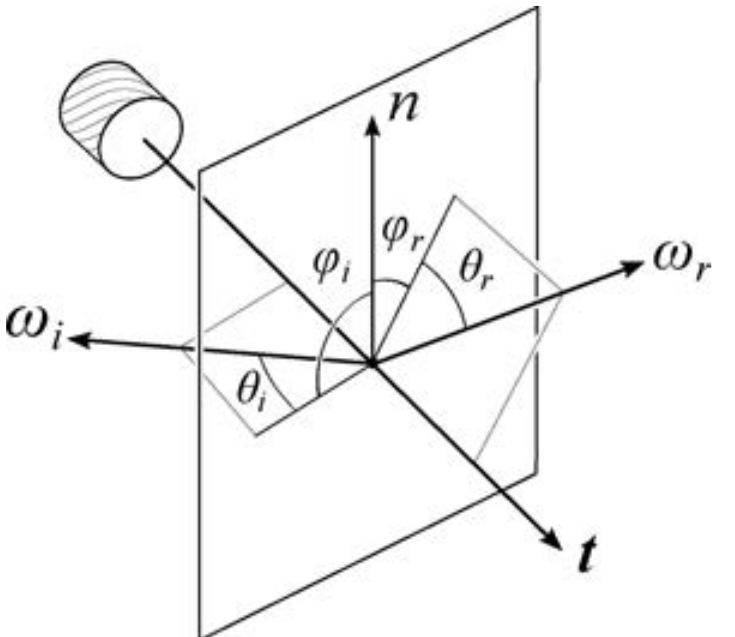
\includegraphics[width=0.35\textwidth]{img/cloth_directions}
\label{fig:cloth_directions}
\end{figure}

\scriptsize{where $f$ is the BRDF function, $t$ is the thread direction, $\omega_i$ is the ray incoming direction, $\omega_r$ is the ray outgoing direction, $F$ are Fresnel terms, $\eta$ are Fresnel coefficients, $\theta$ and $phi$ angles are shown in the figure, $g$ is a Gaussian lobe, $k_d$ is a scattering constant, $A$ is an albedo constant, $\gamma$ are Gaussian widths, $\theta_h = (\theta_i+\theta_r)/2$ and $\phi_d = \phi_i-\phi_r$. }
\end{multicols}

\end{frame}

\subsection{Shading Model}
\begin{frame}{Shading Model}
\begin{figure}[b!]
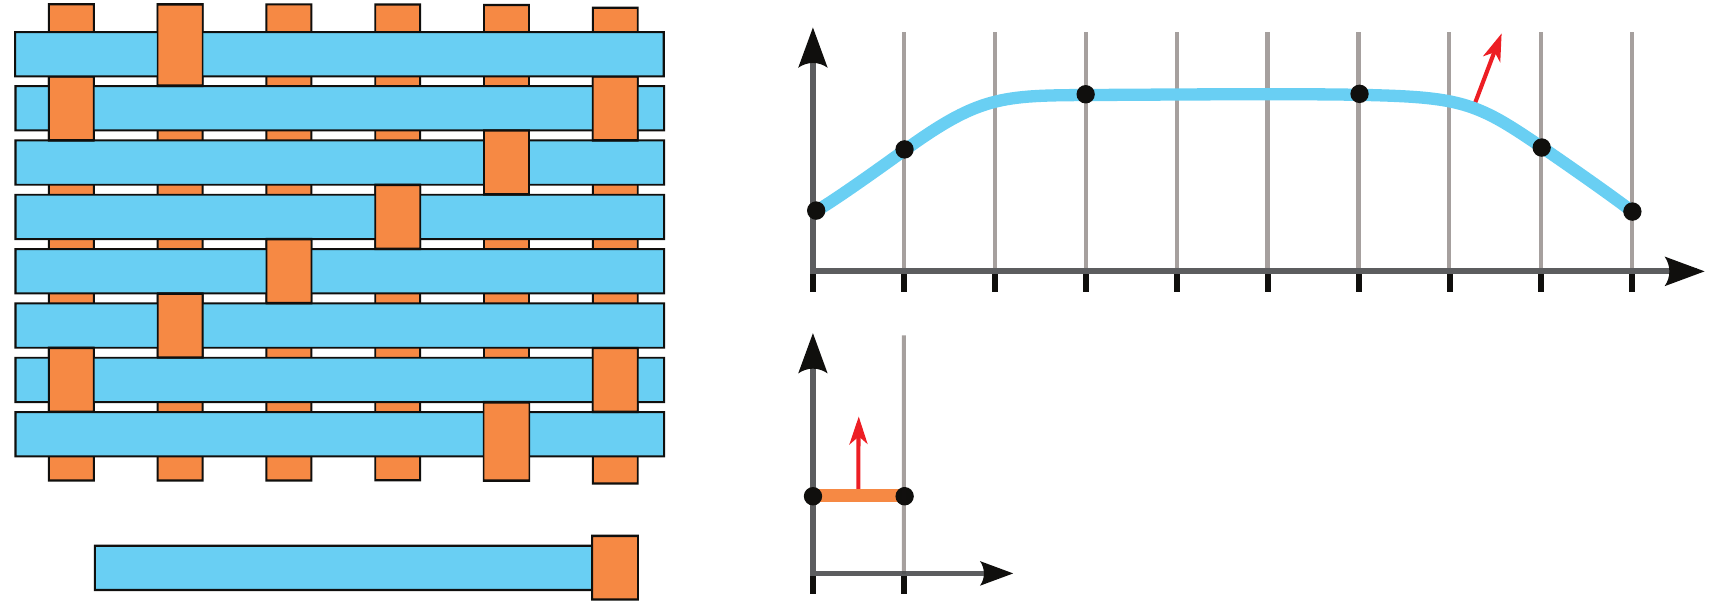
\includegraphics[width=\textwidth]{img/tanget_curve}
\caption*{\tiny{Normal sampling, (top-left) cloth patch, (bottom-left) smallest cloth patch, (top-right) blue thread tangent curve, (bottom-right) red thread tangent curve, image taken from [SBD*13].}}
\end{figure}
\end{frame}

\begin{frame}{Shading Model}
\begin{figure}[b!]
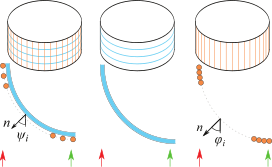
\includegraphics[width=0.8\textwidth]{img/masking}
\caption*{\tiny{Masking examples, Green arrow points view from above, red arrow points view at grazing angle, image taken from [SBD*13].}}
\end{figure}
\end{frame}

\begin{frame}{Shading Model}
\begin{equation*}
L_r(\omega_r) = Q(t) \sum \int L_i(\omega_i) f(t, \omega_i, \omega_r) M(t) P(t) \cos \theta_i d \omega_i,
\end{equation*}

\footnotesize{where $f$ is the BRDF function, $t$ is the thread direction, $\omega_i$ is the ray incoming direction, $\omega_r$ is the ray outgoing direction, $\theta_i$ is the incoming ray angle, $Q(t)$ is a normalization factor for samples and non watertight patches, $M(t)$ is the masking term and $P(t)$ is a view-projection normalization factor.}
\end{frame}

\section{Results and Conclusion}
\subsection{ }

\begin{frame}{Results}

\begin{figure}[!htb]
    \centering
    \begin{minipage}{.48\textwidth}
        \centering
        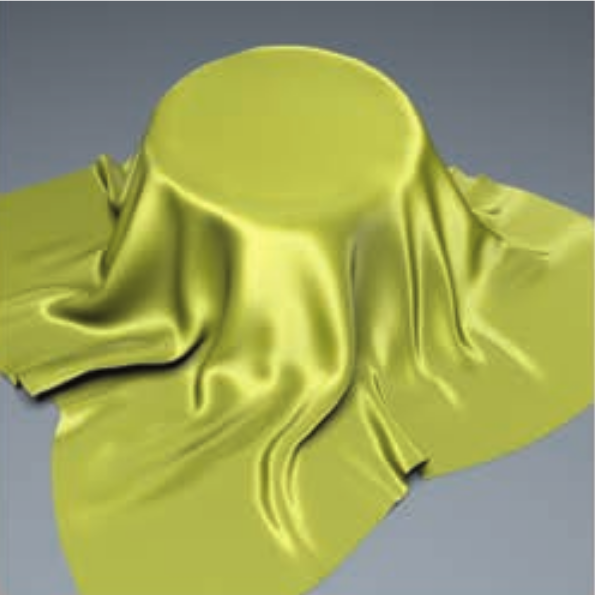
\includegraphics[width=0.8\textwidth]{img/cloth_paper}
        \caption*{Cloth render result from [SBD*13].}
    \end{minipage}%
	\centering
	~
    \begin{minipage}{.48\textwidth}
        \centering
        \movie[width=\textwidth, autostart, loop]
        {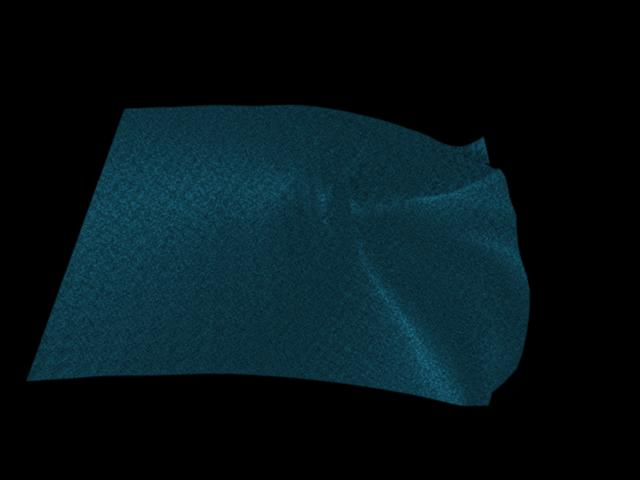
\includegraphics[width=\textwidth]{img/cloth_render}}{img/cloth_render_video.mp4}
        \caption*{Our cloth implementation in Maya\textsuperscript\textregistered using MentalRay\textsuperscript\textregistered.}
    \end{minipage}%    
\end{figure}
\end{frame}

\begin{frame}{Conclusions and Future Work}

\begin{itemize}
\setlength\itemsep{0.5em}
\item Limitations
	\begin{itemize}
	\setlength\itemsep{0.5em}
	\item Requires captured data
	\item Difficult parametrization
	\end{itemize}
\item Future work
	\begin{itemize}
	\setlength\itemsep{0.5em}
	\item Implement full model
	\item Importance sampling extensions by [MI] and [WXK]
	\end{itemize}
\end{itemize}

\end{frame}

\section*{}

\begin{frame}[plain,c]
\begin{center}
\huge Thank you
\\~\\
\Large Questions?
\end{center}

\let\thefootnote\relax\footnotetext{
\textbf{References} \newline \newline
\tiny{
[SBD*13] Sadeghi, I. et al. A practical microcylinder appearance model for cloth rendering. ACM 2013 \newline
[PH10] Pharr, M. et al. Physically based rendering: From theory to implementation, Morgan Kaufmann, 2010 \newline
[MI] Mizutani K. et al. Importance Sampling for Cloth Rendering under Environment Light, Mathematical Progress in Expressive Image Synthesis I, 2014 \newline 
[WXK] Wang J. et al. Importance Sampling for a Microcylinder Based Cloth Bsdf, SIGGRAPH Talks, 2014\\~\\}}
\end{frame}

%----------------------------------------------------------------------

\end{document}
